\documentclass[11pt,twocolumn]{article}
\usepackage[utf8]{inputenc}
\usepackage{graphicx}
\date{}
\usepackage{titlesec}
\usepackage{listings}
\usepackage{subcaption}
\usepackage{amssymb}
\usepackage{amsmath}
\usepackage{float}
\usepackage{subfig}
\usepackage{subcaption}
\usepackage{pgfplots}
\usepackage{tikz}
\usepackage[top=0.5in, bottom=1in, left=1in, right=1.in]{geometry}

\usepackage{titlesec}

\titleformat*{\section}{\large\bfseries}
\titleformat*{\subsection}{\Large\bfseries}
\titleformat*{\subsubsection}{\large\bfseries}
\titleformat*{\paragraph}{\large\bfseries}
\titleformat*{\subparagraph}{\large\bfseries}


\usepackage[english]{babel}
\usepackage[utf8]{inputenc}

\DeclareRobustCommand{\bbone}{\text{\usefont{U}{bbold}{m}{n}1}}
\DeclareMathOperator{\EX}{\mathbb{E}}
\begin{document}
\title{\centerline{\rule{15cm}{2pt}} \textbf{A Survey On Autoencoders}\\\centerline{\rule{15cm}{0.4pt}}}
\author{
  BILICI, M. Şafak\\
  \texttt{safakk.bilici.2112@gmail.com}}
\maketitle
\textbf{\textit{Abstract--}} \textbf{Autoencoders are an unsupervised learning architectures in neural networks. Theys are commonly used in Deep Learning tasks; such as generative models, anomaly detection, dimensionality reduction. In this article, we will evaluate theoretical approaches of Autoencoders and see it's extensions.}

\section{1 Introduction}
\hspace*{0.5cm} Autoencoders are an unsupervised learning method. They map the input data into lower dimensional space with encoder $E$, and then maps into same space that have same dimension of input data with decoder $D$.\\
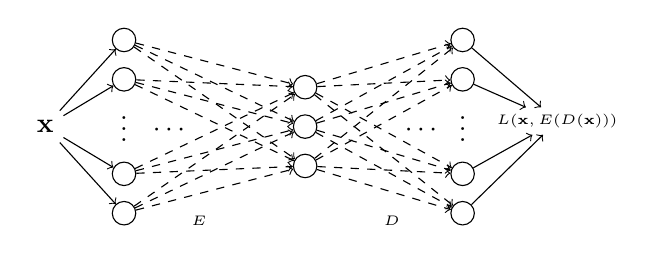
\begin{tikzpicture}

      \node[inner sep=3pt] (z) at (-0.4,-1.15){$\cdots$};
      \node[circle,draw=black,minimum size=0.2cm,inner sep=3pt] (a) at (-1,0){};
      \node[circle,draw=black,minimum size=0.1cm,inner sep=3pt] (b) at (-1,-0.5){};
      
      \node[] (e) at (0.2,0){};
      \node[circle,draw=black,minimum size=0.1cm,inner sep=3pt] (f) at (1.3,-0.6){};
      \node[circle,draw=black,minimum size=0.1cm,inner sep=3pt] (g) at (1.3,-1.1){};
      \node[circle,draw=black,minimum size=0.1cm,inner sep=3pt] (h) at (1.3,-1.6){};
      
      \node[inner sep=3pt] (z) at (-1,-1.03){$\vdots$};
     
      \node[circle,draw=black,minimum size=0.1cm,inner sep=3pt] (c) at (-1,-1.7){};
      \node[circle,draw=black,minimum size=0.1cm,inner sep=3pt] (d) at (-1,-2.2){};
      \node[] (w) at (-2,-1.1){$\mathbf{x}$};
      \node[inner sep=3pt] (o) at (2.8,-1.15){$\cdots$};
      \node[circle,draw=black,minimum size=0.2cm,inner sep=3pt] (i) at (3.3,0){};
      \node[circle,draw=black,minimum size=0.1cm,inner sep=3pt] (j) at (3.3,-0.5){};
      \node[inner sep=3pt] (m) at (3.3,-1.03){$\vdots$};
      \node[circle,draw=black,minimum size=0.1cm,inner sep=3pt] (k) at (3.3,-1.7){};
      \node[circle,draw=black,minimum size=0.1cm,inner sep=3pt] (l) at (3.3,-2.2){};
      \tiny
      \node[] (n) at (4.5,-1.03){$L(\mathbf{x},E(D(\mathbf{x})))$};
      
      \node[inner sep=3pt] (p) at (-0.05,-2.3){$E$};
      \node[inner sep=3pt] (r) at (2.4,-2.3){$D$};
      
      \draw[->] (w) -- (a);
      \draw[->] (w) -- (b);
      \draw[->] (w) -- (c);
      \draw[->] (w) -- (d);
      \draw[dashed,->] (a) -- (f);
      \draw[dashed,->] (a) -- (g);
      \draw[dashed,->] (a) -- (h);
      \draw[dashed,->] (b) -- (f);
      \draw[dashed,->] (b) -- (g);
      \draw[dashed,->] (b) -- (h);
      \draw[dashed,->] (c) -- (f);
      \draw[dashed,->] (c) -- (g);
      \draw[dashed,->] (c) -- (h);
      \draw[dashed,->] (d) -- (f);
      \draw[dashed,->] (d) -- (g);
      \draw[dashed,->] (d) -- (h);
      \draw[dashed,->] (f) -- (i);
      \draw[dashed,->] (f) -- (j);
      \draw[dashed,->] (f) -- (k);
      \draw[dashed,->] (f) -- (l);
      \draw[dashed,->] (g) -- (i);
      \draw[dashed,->] (g) -- (j);
      \draw[dashed,->] (g) -- (k);
      \draw[dashed,->] (g) -- (l);
      \draw[dashed,->] (h) -- (i);
      \draw[dashed,->] (h) -- (j);
      \draw[dashed,->] (h) -- (k);
      \draw[dashed,->] (h) -- (l);
      \draw[->] (i) -- (n);
      \draw[->] (j) -- (n);
      \draw[->] (k) -- (n);
      \draw[->] (l) -- (n);
    \end{tikzpicture}
The main idea behind Autoencoders is to attempt to copy its input to its output. The input layer is fed with input vector $\mathbf{x}$ and the loss is calculated at output layer between $\mathbf{x}$ and $E(D(\mathbf{x}))$, in other words the loss is $L(\mathbf{x},E(D(\mathbf{x})))$. It measures difference between our original input and the consequent reconstruction.  We named the middle layer, that is connection between encoder $E$ and decoder $D$, as the "bottleneck". We can denote our output of bottleneck as $\mathbf{h} = E(\mathbf{x})$ and denote our output as $\mathbf{\hat{x}} = D(\mathbf{h}) = D(E(\mathbf{x}))$. We can define our encoder and decoder as conditional probability density function that are $p_{encoder}(\mathbf{h} | \mathbf{x})$ and $p_{decoder}(\mathbf{\hat{x}} | \mathbf{h})$. \\
The loss function is named reconstruction loss which is $L(\mathbf{\hat{x}},\mathbf{x})$. We can treat the process as a feedforward networks; the loss can be minimized via mini-batch statistics following gradients computed by backpropagation algorithm,
$$\min\limits_{\theta} L = \nabla_\theta L(\mathbf{x}, E(D(\mathbf{x}))) =\nabla_\theta L(\mathbf{x}, \mathbf{\hat{x}}) $$
The bottleneck is the key of the effectiveness of Autoencoders. We map our input vector to bottleneck: the bottleneck keeps the 'latent informations' of input $\mathbf{x}$. The network represents input but in lower dimensions. In other words, it behaves like a approximative compression algorithm. The encoding parameters are learned in training process. Then we map bottleneck information $\mathbf{h}$ into same dimension as input $\mathbf{x}$. Then, this procedure can be seen as approximative extracting compressed latent information.

\section{2 Undercomplete Autoencoders}

\end{document}